%\documentclass{uai2021} % for initial submission
 \documentclass[accepted]{uai2021} % after acceptance, for a revised
                                    % version; also before submission to
                                    % see how the non-anonymous paper
                                    % would look like
% NOTE: Only comment/uncomment the lines above as appropriate,
%       as they will be replaced automatically for papers to be published.
%       Do not make any other change above this note for an accepted
%       version.

%% Choose your variant of English; be consistent
\usepackage[american]{babel}
% \usepackage[british]{babel}

%% Some suggested packages, as needed:
\usepackage{natbib} % has a nice set of citation styles and commands
    \bibliographystyle{plainnat}
    \renewcommand{\bibsection}{\subsubsection*{References}}
\usepackage{mathtools} % amsmath with fixes and additions
% \usepackage{siunitx} % for proper typesetting of numbers and units
\usepackage{booktabs} % commands to create good-looking tables
\usepackage{tikz} % nice language for creating drawings and diagrams

%%%%%%%%%%%%%%%%%%%%%%%%%%%

\usepackage{amsthm}

%%%%%%%%%%%%%%%%%%%%%%%%%%%

%% Provided macros
% \smaller: Because the class footnote size is essentially LaTeX's \small,
%           redefining \footnotesize, we provide the original \footnotesize
%           using this macro.
%           (Use only sparingly, e.g., in drawings, as it is quite small.)

%% Self-defined macros
\newcommand{\swap}[3][-]{#3#1#2} % just an example


%%%%%%%%%%%%%%%%%%%%%%%%%%%

\newtheorem{thm}{Theorem}
\newtheorem{algo}[thm]{Algorithm}
\newtheorem{ass}[thm]{Assumption}
\newtheorem{cor}[thm]{Corollary}
\newtheorem{defn}[thm]{Definition}
\newtheorem{exmp}[thm]{Example}
\newtheorem{lem}[thm]{Lemma}
\newtheorem{prop}[thm]{Proposition}
\newtheorem{rem}[thm]{Remark}


\newcommand{\pa}{\textnormal{pa}}

\newcommand{\ds}{\text{ds}}
\newcommand{\dt}{\text{dt}}

\newcommand{\disjU}{\mathbin{\dot{\cup}}}

\usepackage{tikz}
\usepgflibrary{arrows}
\usetikzlibrary{shapes}
\usetikzlibrary{arrows.meta}
\usetikzlibrary{positioning}

\usepackage{graphicx}
\usepackage{caption}
\usepackage{subcaption}


%%%%%%%%%%%%%%%%%%%%%%%%%%%


\title{Equality Constraints and Causal Identification in Linear Hawkes 
Processes}

% The standard author block has changed for UAI 2021 to provide
% more space for long author lists and allow for complex affiliations
%
% All author information is authomatically removed by the class for the
% anonymous submission version of your paper, so you can already add your
% information below.
%
% Add authors in order of decreasing contribution
\author[1]{\href{mailto: Søren Wengel Mogensen 
<swemo@dtu.dk>}{Søren~Wengel~Mogensen}{}} 
% Add affiliations after the authors
\affil[1]{%
    Section of Cognitive Systems\\
    Technical University of Denmark\\
    Denmark
}

\begin{document}
\maketitle

\begin{abstract}
  This is the abstract for this article.
  It should give a self-contained single-paragraph summary of the article's contents, including context, results, and conclusions.
  Avoid citations; but if you do, you must give essentially the whole reference.
  For example: This whole paper is devoted to praising É. Š. Åland von Vèreweg's most recent book (“Utopia's government formation problems during the last millenium”, Springevier Publishers, 2016).
  Also, do not put mathematical notation and abbreviations in your abstract; be descriptive.
  So not “we solve \(x^2+A xy+y^2\), where \(A\) is an RV”, but “we solve quadratic equations in two unknowns in which a single coefficient is a random variable”.
  The reason is that mathematical notation will not display correctly when the abstract is reused on the proceedings website, for example, and that one should not assume the abstract's reader knows the abbreviation.
  Of course the same remarks hold for your paper's title.
\end{abstract}

Main focus on equality constraints: follows from parametric form of integrated 
cumulative variance matrix, biproduct: HTC-type identification results follow, 
give example of equality constraint using dynamical information (check that 
there are no equality constraints in this case using only integrated matrix)

add also soft intervention interpretation of the Hawkes processes

\section{Introduction}\label{sec:intro}

In classical work, conditional independence has been used as a testable 
implication of causal models. In addition, equality constraints (or Verma, or 
dormant, same thing?) have been proposed to distinguish between data-generating 
mechanisms. In stochastic processes, local independence is a concept which can 
be used analogous to conditional independence. In this paper, we show that one 
can also find equality constraints in the class of linear Hawkes process that 
have been a much studied model class recently in machine learning. We show that 
these class of models in a certain sense satisfy the same equality constraints 
as a cyclic linear structural equation model, and we also show that one may 
find additional constraints using when the process is observed over time.

This also naturally leads to new identification results for Hawkes processes, 
and we also give a causal interpretation of the parameters which is closely 
related to the so-called cluster representation of a linear Hawkes process.



%%%%%%%%%%%%%%%%%%%%%%%%%%%
%%%%%%%%%%%%%%%%%%%%%%%%%%%

\section{Hawkes Processes}

\begin{defn}[Linear Hawkes process]
	We say that a point process, $N$, is a \emph{linear Hawkes process} if the 
	intensity is of the form
	
	$$
	\lambda_t^\beta = \mu_\beta + \sum_{\beta \in V} \int_{-\infty}^{t} 
	g_{\beta\alpha}(t - s) d 
	N_s^\alpha
	$$
	
	\noindent for all $\beta\in V$ and $t\in R$. 
	\label{def:hawProc}
\end{defn}

We will often refer to a linear Hawkes process by just saying Hawkes process. 
We assume throughout that $g_{\beta\alpha}$ is a continuous function for all 
$\alpha$ and $\beta$ and that the coordinate processes of the Hawkes 
process are indexed by the set $V = \{1,2,\ldots, n\}$.

We define the $n\times n$ matrix $G$ such that $G_{\beta\alpha} = 
\int_{-\infty}^\infty 
g_{\beta\alpha}(s) \ds$. We assume that the spectral radius of $G$ (largest 
absolute value of its eigenvalues) is less than 1 which implies that we can 
assume the Hawkes process to be stationary \citep{jovanovic2015}.
We define $n\times n$ matrix $R=(I_n - G)^{-1}$ where $I_n$ is the 
$n\times n$ identity matrix. This is well-defined due to the assumption on 
the spectral radius of $G$ and furthermore $R = \sum_{i=0}^\infty G^i$. 

We will introduce two statistical concepts that we will use in our results. One 
is seen to be an integrated (and time-independent) measure of covariance and 
one is seen to be a 
time-dependent measure of covariance.

%%%%%%%%%%%%%%%%%%%%%%%%%%%

\paragraph{Infinitesimal Covariance}

For a $n$-dimensional stationary point process, we define the intensity vector 
(mean vector?), following [Hawkes JRSS-B, 1971]

$$
\lambda = E(dN(t))/dt
$$

\noindent and covariance density matrix

$$
k(\tau) = 
$$

[see Hawkes JRSS-B, 1971 - compare this to bacry and muzy]

%%%%%%%%%%%%%%%%%%%%%%%%%%%

\paragraph{Integrated Covariance}

We can integrate the infinitesimal covariance over time to obtain a type of 
integrated cumulant matrix, $C$. This matrix satisfies the equation

$$
C = R \Lambda R^T,
$$

see \cite{jovanovic2015}.

%%%%%%%%%%%%%%%%%%%%%%%%%%%

\paragraph{Cluster Representation}

In Definition \ref{def:hawProc}, Hawkes processes are introduced by specifying 
the intensity processes. One can also define them by using a so-called cluster 
representation which, as we will see, lends itself to a straight-forward causal 
interpretation. [this is complicated by the doubly-infinite nature of the 
process? not started at zero]




%%%%%%%%%%%%%%%%%%%%%%%%%%%
%%%%%%%%%%%%%%%%%%%%%%%%%%%

\subsection{Causal Interpretation}

In this section, we will define what we mean by a {\it causal} Hawkes process.

[ref] gave a causal interpretation using hard interventions. We instead give an 
interpretation using what can be thought of as \emph{soft interventions}. Each 
generation 0 node has an associated 'Hawkes tree', i.e., the nodes that are 
descendants in the generating process (note that this is different from 
descendants in the causal graph). We say that [language] this is causal Hawkes 
process if 

$$
\bar{N} = 
$$

$$
P_\alpha = P_{\bar{\alpha}}
$$

for all coordinate processes $\alpha \in V$. In words, the intervention events 
propagate in the same way through the system as the intrinsic events. This 
corresponds to how interventions could be undertaken in some fields of science, 
e.g., in neuroscience where in some experiments on can incur a change in the 
action potential for some neurons, however not change their inner dynamics nor 
sever causal parents [ref]. This assumption is seen to correspond closely to 
the \emph{modularity} assumption which is often underpins the causal 
interpretation of structural causals models [ref] in that the mechanism which 
governs the data generation is the same in both observational and 
interventional settings. In the Hawkes process model this can be translated 
into the assumption that each Hawkes tree develops in the same way, regardless 
of whether the root event (the generation 0 event) is interventional or not.

\begin{defn}[Causal effects]
	We will say that $G_{\beta\alpha}$ is the {\it direct causal effect} from 
	$\alpha$ on $\beta$ and that $R_{\beta\alpha}$ is the {\it total causal 
	effect} from $\alpha$ on $\beta$. We will say that $g_{\beta\alpha}$ is the 
	{\it causal function} from $\alpha$ to $\beta$.
	\label{def:cauEff}
\end{defn}

From the above definition and the causal assumption, the interpretation of 
direct and total causal effects is straight-forward: if we were to inject an 
interventional event of type $\alpha$ at time $s \in R$, then this 
would on average lead (directly, first generation) to $G_{\beta\alpha}$ events 
of type $\beta$ (when considering all $t > s$). The Hawkes tree rooted at the 
interventional $\alpha$ event would in total have $R_{\beta\alpha}$ events of 
type $\beta$ (does this also hold for alpha = beta?) [write also as a formula, 
equation?]

One could of course also think of $g_{\beta\alpha}$ as a causal effect, or 
describing one.

Under the causal assumption that we make, we see that the above are \ldots

%%%%%%%%%%%%%%%%%%%%%%%%%%%

\paragraph{Graphical representation}

A {\it graph} is a pair $(V,E)$ where $V$ is a finite set of nodes and $E$ is a 
set edges, each between a pair of (not necessarily distinct) nodes. We will 
only consider {\it directed graphs}, i.e., graphs such that every node is of 
the type, $\rightarrow$.

Given a Hawkes process with coordinate processes indexed by $V = 
\{1,2,\ldots,n\}$, we construct its graph, $\mathcal{D} = (V,E)$, such that 
$\alpha \rightarrow_\mathcal{D} \beta$ if and only if $g_{\beta\alpha} \neq 0$. 
We say that $\mathcal{D}$ is the {\it causal graph} of the Hawkes process.


%%%%%%%%%%%%%%%%%%%%%%%%%%%
%%%%%%%%%%%%%%%%%%%%%%%%%%%

\section{Identification}

In this paper, we will mostly focus on the identification of the entries in the 
matrix $R$, and of G?. We will say that some object, $i$, is identified from 
$f(P)$ where 
$P$ is the distribution of a stationary Hawkes process if $f(P_1) = f(P_2)$ 
implies $i_1 = i_2$. [check definition]

%%%%%%%%%%%%%%%%%%%%%%%%%%%

\subsection{Identifying direct causal effect}

The Hawkes processes are an infinite-dimensional family and this approach also 
shows that equality constraints are retained even in the finite-dimensional 
integrated cumulants which makes it easier to use in practical structure 
learning.

[for this we can use half-trek arguments?]

We will introduce the matrix $\tilde{G}$ by scaling each column of $G$ by its 
diagonal element and placing zeros on the diagonal, i.e.,

$$
\tilde{g}_{ij} = g_{ij}/g_{jj}  \text{ if } i\neq j, \text{ and } 
\tilde{g}_{ij} 
= 0 \text{ if } i= j.
$$

[this scaling is actually also in the Hyttinen et al. paper] Let $D$ denote a 
diagonal matrix such that the $i$'th diagonal element equals 
$1 - g_{ii}$. This means that 

$$
\Sigma = (I - G)\Lambda (I - G)^T = (I - \tilde{G})D \Lambda D(I - \tilde{G})^T.
$$

The type of equation is well-studied in the context of linear structural 
equation models [refs] and we can use available results to argue about 
identifiability of the parameters in $\tilde{G}$ and $G$. Note that while this 
casts the Hawkes identification as a set of equations describing the covariance 
matrix of a linear structural equation model, this is not a reparametrization 
of the latter as there are constraints on the the Hawkes parameters (spectral 
and nonnegativity of entries in $G$).


\subsubsection{Marginalization}

We will mostly be interested in systems that are only partially observed in 
which case only a proper submatrix of $\Sigma$ is observed. We let $V = O \cup 
U$. Assume that $\bar{\Sigma}$ is the observed submatrix [argue that this 
actually only uses the marginal distribution of the observed processes] We have 
that 

\begin{align}
\bar{\Sigma} = (I - \bar{G})\Theta(I - \bar{G})^T
\end{align}

where 

\begin{align*}
\bar{G} & = \\
\Theta & = 
\end{align*}

We say that $\alpha \rightarrow \gamma_1 \rightarrow \ldots \rightarrow 
\gamma_k \rightarrow \beta$ is an \emph{unobserved} directed path from $\alpha$ 
to $\beta$ if $\gamma_i \in U$ for all $i = 1,\ldots, k$. 

\begin{prop}
	Let $\alpha,\beta \in O$. The parameter $\tilde{G}_{\beta\alpha}$ is 
	identified 
	from the integrated first- and second order moments [define these] if there 
	are no unobserved directed paths [maybe this should be walks - then also 
	works for alpha = beta, then gives the next corollay directly?] from 
	$\alpha$ to $\beta$ and [HTC criterion]. The parameter $G_{\beta\alpha}$ is 
	identified if $\tilde{G}_{\beta\alpha}$ and $\tilde{G}_{\beta\beta}$ (no 
	this is zero, maybe if something in theta is identified?) are 
	identified.
\end{prop}

[HTC is actually generic identifiability, not global identifiability!]

\begin{proof}
	content...
\end{proof}

\begin{cor}
	[something about id of parameters in G]
\end{cor}

%%%%%%%%%%%%%%%%%%%%%%%%%%%

\subsection{Identifying total causal effect}

From the integrated covariance matrix (name?), depending on the graphical 
structure, we may obtain identification of some of the entries in $R$. We know 
that 

\begin{align*}
	C & = R \Lambda R^T \\
	& = S S^T
\end{align*}

\noindent where $S = R\Lambda^{1/2}$. The diagonal matrix $\Lambda^{1/2}$ is 
the entrywise squareroot of $\Lambda$. 

This is similar to the Gaussian linear structural equation model [ref] and we 
can prove that similar identification results hold. [what we need is to argue 
about the unobserved nodes]

%%%%%%%%%%%%%%%%%%%%%%%%%%%

\subsection{Identifying causal functions}

It is only natural that we can obtain stronger identification results when we 
use more aspects of the distribution. [only stationary hawkes, needed for the 
next result?]

\begin{prop}
	Let $\mathcal{D} = (O\disjU U, E)$. If $\pa_\mathcal{D}(\alpha) \subseteq 
	O$, then for all $\beta$ the function $g_{\alpha\beta}$ is identified from 
	the covariance process of $O$-processes.
	\label{prop:gPaId}
\end{prop}



\begin{proof}
	1
\end{proof}

%%%%%%%%%%%%%%%%%%%%%%%%%%%
%%%%%%%%%%%%%%%%%%%%%%%%%%%

\section{Equality constraints}

In causal models, it is well-known that the structure imposes constraints that 
are not described by conditional independence. Local independence (see 
Definition \ref{def:li}) has been used analogously in stochastic processes and 
the obvious question is therefore whether there are constraints imposed by the 
structure that are not described by local independence. This is indeed the case 
and moreover, one can use the integrated cumulants to find such examples.

\begin{defn}[Local independence]
	\label{def:li}
\end{defn}

From rewriting the equation into using $\tilde{G}$ we see that the equality 
constraints in a linear structural equation model impose the same constraints 
on the parameters $(\tilde{G}, \Theta)$ and this allows us to find constraints 
in the Hawkes process. We will show by an example that these constraints may 
provide information about the underlying structure that is not contained the 
Markov equivalence class.

\subsection{Integrated cumulants}

\subsection{Dynamical cumulants}

Q: is everything always id'ed in R using dynamical info? probably not, take a 
complete graph with something unobserved?

In this subsection, we will simply give an example where one can obtain 
additional identification, and an additional equality constraint, using 
dynamical observation as compared to only using the . From Proposition 
\ref{prop:gPaId}, it follows that

\begin{exmp}
	
	\begin{figure*}
		%\begin{tabular}{cc}
		\begin{subfigure}{0.48\linewidth}
			\centering
			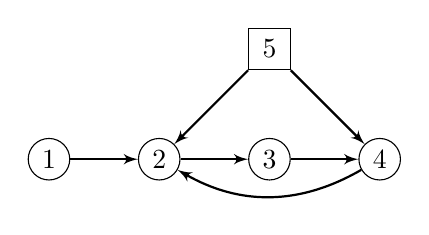
\begin{tikzpicture}[scale=0.7]
			\tikzset{vertex/.style = {shape=circle,draw,minimum size=1.5em, 
			inner 
					sep = 0pt}}
			\tikzset{edge/.style = {->,> = latex', thick}}
			\tikzset{edgebi/.style = {<->,> = latex', thick}}
			\tikzset{every loop/.style={min distance=8mm, looseness=5}}
			\tikzset{vertexFac/.style = {shape=rectangle,draw,minimum 
			size=1.5em, 
					inner sep = 0pt}}
			
			% vertices
			%\draw [line width=35pt,opacity=0.1, blue,line cap=round,rounded
			%corners] (0,0.5) -- (0,2) -- (-1.5,1.5) -- (0,0.5);
			\node[vertex] (a) at  (-4,0) {$1$};
			\node[vertex] (b) at  (-2,0) {$2$};
			\node[vertex] (c) at  (0,0) {$3$};
			\node[vertex] (d) at  (2,0) {$4$};
			\node[vertexFac] (e) at  (0,2) {$5$};
			
			%edges
			
			\draw[edge] (a) to (b);
			\draw[edge] (b) to (c);
			\draw[edge] (c) to (d);
			\draw[edge, bend left = 30] (d) to (b);
			\draw[edge] (e) to (d);
			\draw[edge] (e) to (b);
			
			\end{tikzpicture}
		\end{subfigure}
		\begin{subfigure}{0.48\linewidth}
			\centering
			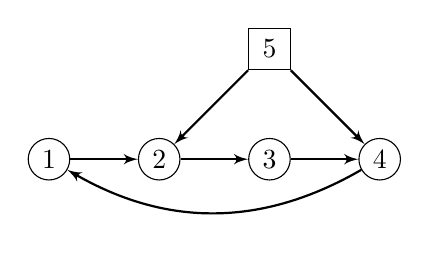
\begin{tikzpicture}[scale=0.7]
			\tikzset{vertex/.style = {shape=circle,draw,minimum size=1.5em, 
					inner 
					sep = 0pt}}
			\tikzset{edge/.style = {->,> = latex', thick}}
			\tikzset{edgebi/.style = {<->,> = latex', thick}}
			\tikzset{every loop/.style={min distance=8mm, looseness=5}}
			\tikzset{vertexFac/.style = {shape=rectangle,draw,minimum 
					size=1.5em, 
					inner sep = 0pt}}
			
			% vertices
			%\draw [line width=35pt,opacity=0.1, blue,line cap=round,rounded
			%corners] (0,0.5) -- (0,2) -- (-1.5,1.5) -- (0,0.5);
			\node[vertex] (a) at  (-4,0) {$1$};
			\node[vertex] (b) at  (-2,0) {$2$};
			\node[vertex] (c) at  (0,0) {$3$};
			\node[vertex] (d) at  (2,0) {$4$};
			\node[vertexFac] (e) at  (0,2) {$5$};
			
			%edges
			
			\draw[edge] (a) to (b);
			\draw[edge] (b) to (c);
			\draw[edge] (c) to (d);
			\draw[edge, bend left = 30] (d) to (a);
			\draw[edge] (e) to (d);
			\draw[edge] (e) to (b);

			
			\end{tikzpicture}
		\end{subfigure}
		%\end{tabular}
		\caption{\label{fig:cyclicDGs} Loops (self-edges) are omitted from this 
		vizualiation. Circles represent observed coordinate processes and 
		squares represent unobserved processes. Left: . Right: }
	\end{figure*}
	
	We consider the graph in Figure \ref{fig:cyclicDGs} (right). When 5 is 
	unobserved, we cannot in general identify any entries of $R$ or of $G$ from 
	the integrated covariances ($C$) [make argument, and find example to show 
	this - what is actually not id'ed? Both R's and G's, or just G's???]. 
	Instead we assume in this example that we also have access to the 
	covariance processes. In this case, the causal functions 
	$g_{11},g_{41},g_{23}$, and $g_{33}$ are identified (Proposition 
	\ref{prop:gPaId}), and therefore so are $G_{11}, G_{41} , G_{23}$ and 
	$G_{33}$.
\end{exmp}


%%%%%%%%%%%%%%%%%%%%%%%%%%%
%%%%%%%%%%%%%%%%%%%%%%%%%%%

\section{Conclusion}

A Hawkes process is defined using the set of $g_{\beta\alpha}$-functions along 
with the $\mu_\alpha$-constants for $\alpha,\beta$ in the finite set $V$. The 
constraints that are shown to exist in this paper are not the only constraints 
imposed by the distribution of the Hawkes process [do I actually know this?] On 
the other hand, they seem to offer also a dimension reduction in that we 
actually test these constraints using a finite parameter space instead of a 
function space. This should make them more suitable to employ in data analysis, 
seeing estimation of $g$ is a challenging problem even in the case of full 
observation [cite recent work] and partial observation only adds to the 
complexity of this task [cite nicolajs thesis]. This approach partially 
circumvents this problem (ref also Achab's paper).


%%%%%%%%%%%%%%%%%%%%%%%%%%%
%%%%%%%%%%%%%%%%%%%%%%%%%%%


\section{General Formatting Instructions}
As a general rule: \emph{follow the template}.

\subsection{Authorship}
Reviewing is double-blind.
However, you can already fill in your author names and affiliations in the \verb|\author| block in the preamble following the example of the template because the class will remove it as long as the option \textsf{accepted} is not passed to the class.
Nevertheless, make sure any other information in the paper does not disclose your identity, for example URLs to supplementary material.

\subsection{Sectioning}
Three numbered sectioning commands are provided: \verb|\section|, \verb|\subsection|, and \verb|\subsubsection|.
Please respect their order, so do not put a \verb|\subsubsection| directly beneath a \verb|\section|.
One unnumbered sectioning command is provided, \verb|\paragraph|.
It can be used directly below any numbered section level.
Do not use any other sectioning commands.

\subsubsection{Typing the Section Titles}
The \verb|\section| and \verb|\subsection| titles are uppercased by the class.
Please type them in title case.
(This is used in the PDF bookmarks.)
Please also write the \verb|\subsubsection| titles in title case.

\paragraph{What is title case?}
\href{https://en.wikipedia.org/wiki/Title_case}{Wikipedia} explains:
\begin{quote}
    Title case or headline case is a style of capitalization used for rendering the titles of published works or works of art in English.
    When using title case, all words are capitalized except for ‘minor’ words (typically articles, short prepositions, and some conjunctions) unless they are the first or last word of the title.
\end{quote}

\subsection{References, Citations, Footnotes}\label{sec:etc}
\subsubsection{Cross-Referencing}
Always use \verb|\label| and \verb|\ref|—or a command with a similar effect—when cross-referencing.
For example, this subsection is Section~\ref{sec:etc}.

\subsubsection{Citations}
Citations should include the author's last name and year.
They should be part of the sentence.
An example parenthetical citation: “Good introductions to the topic are available \citep{latexcompanion}.”
An example textual citation: “\citet{einstein} discusses electrodynamics of moving bodies.”
Do not use a parenthetical citation where a textual one is appropriate.
An example of what \emph{not} to do: “\citep{einstein} discusses electrodynamics of moving bodies.”

We strongly advise to use reference list software such as Bib\TeX{} and a citation package such as \textsf{natbib}.
The reference style you use should be compatible with the author-year citations.
Both the citation style and reference style used should be consistent.

For the original submission, take care not to reveal the authors' identity through the manner in which one's own previous work is cited.
For example, writing
“I discussed electrodynamics of moving bodies before \citep{einstein}.” would be inappropriate, as it reveals the author's identity.
Instead, write “\citet{einstein} discussed electrodynamics of moving bodies.”

\subsubsection{Footnotes}
You can include footnotes in your text.\footnote{
    Use footnotes sparingly, as they can be distracting, having readers skip back and forth between the main text and the foot of the page.
}
The footnote mark should follow the fragment to which it refers, so a footnote\footnote{
    A footnote is material put at the foot of a page.
}
for a word has a footnote mark attached to that word and a footnote for a phrase or sentence has a footnote mark attached to the closing punctuation.

\section{Math}\label{sec:math}
The class file does not load any math support package like \textsf{amsmath}\footnote{%
  See the \textsf{amsmath} documentation at \url{https://ctan.org/pkg/amsmath} for further details.
}.
We advise using the \textsf{mathtools}\footnote{%
  See the \textsf{mathtools} documentation at \url{https://ctan.org/pkg/mathtools} for further details.
}
package, which extends \textsf{amsmath} with fixes and even more useful commands.
Feel free to load other support packages for symbols, theorems, etc.

Use the \textsf{amsmath} environments for displayed equations.
So, specifically, use the \texttt{equation} environment instead of \verb|$$...$$| and the \texttt{align} environment instead of \texttt{eqnarray}.\footnote{For reasons why you should not use the obsolete \texttt{eqnarray} environment, see Lars Madsen, \textit{Avoid eqnarray!} TUGboat 33(1):21--25, 2012.}
An \texttt{equation}:
\begin{equation}\label{eq:example}
  0 = 1 - 1.
\end{equation}
Two \texttt{align}'ed equations:
\begin{align*} % no numbers with starred version
  1 + 2 &= 3,\\
  1 - 2 &= -1.
\end{align*}
Equations can also be put inline, of course.
For example, Equation~\eqref{eq:example}: \(0=1+1\). % $0=1+1$ also works
(Notice that both inline and displayed math are part of the sentence, so punctuation should be added to displayed math.)

The \textsf{amsmath} and \textsf{mathtools} packages provide a lot of nice functionality, such as many common math operators, e.g., \(\sin\) and \(\max\), and also commands for defining new ones.

\section{Floats}\label{sec:floats}
Floats, such as figures, tables and algorithms, are moving objects and are supposed to float to the nearest convenient location.
Please do not force them to go in the middle of a paragraph.
They must respect the column width.

Two-column floats are possible.
They appear at the top of the next page, so strategic placement may be necessary.
For an example, see Figure~\ref{fig:tikz}.
They may not enter the margins.
\begin{figure*}
    \centering
    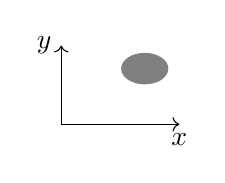
\begin{tikzpicture}[xscale=1.5]
        \coordinate (origin);
        \draw[->] (origin) -- +(1cm,0) node[below] {$x$};
        \draw[->] (origin) -- +(0,1cm) node[left] {$y$};
        \fill[gray] (45:1cm) circle[radius=.2cm];
    \end{tikzpicture}
    \caption{A Nice Filled Ellipse with a Pair of Coordinate Axes.}\label{fig:tikz}
\end{figure*}

All material in floats should be legible and of good quality.
So avoid very small or large text and pixelated or fuzzy lines.

\subsection{Figures}\label{sec:figures}
Figures should go in the \texttt{figure} environment and be centered therein.
The caption should go below the figure.
Use \verb|\includegraphics| for external graphics files but omit the file extension.
Supported formats are \textsf{pdf} (preferred for vector drawings and diagrams), \textsf{png} (preferred for screenshots), and \textsf{jpeg} (preferred for photographs).
Do not use \verb|\epsfig| or \verb|\psfig|.
If you want to scale the image, it is better to use a fraction of the line width rather than an explicit length.
For example, see Figure~\ref{fig:toronto}.
\begin{figure}
  \centering
  \includegraphics[width=0.7\linewidth,page=3]{toronto}
  \caption{A View of a Nice City.}\label{fig:toronto}
\end{figure}

Do not use \verb|\graphicspath|.
If the images are contained in a subdirectory, specify this when you include the image, for example \verb|\includegraphics{figures/mypic}|.

\subsection{Tables}\label{sec:tables}
Tables should go in the \texttt{table} environment and be centered therein.
The caption should go above the table and be in title caps.
For an example, see Table~\ref{tab:data}.
\begin{table}
    \centering
    \caption{An Interesting Table.}\label{tab:data}
    \begin{tabular}{rl}
      \toprule % from booktabs package
      \bfseries Dataset & \bfseries Result\\
      \midrule % from booktabs package
      Data1 & 0.12345\\
      Data2 & 0.67890\\
      Data3 & 0.54321\\
      Data4 & 0.09876\\
      \bottomrule % from booktabs package
    \end{tabular}
\end{table}

\subsection{Algorithms}\label{sec:algorithms}
You can load your favorite algorithm package, such as \textsf{algorithm2e}\footnote{See the \textsf{algorithm2e} documentation at \url{https://ctan.org/pkg/algorithm2e}.}.
Use the environment defined in the package to create a centered float with an algorithm inside.

\section{Back Matter}
There are a some final, special sections that come at the back of the paper, in the following order:
\begin{itemize}
  \item Author Contributions
  \item Acknowledgements
  \item References
\end{itemize}
They all use an unnumbered \verb|\subsubsection|.

For the first two special environments are provided.
(These sections are automatically removed for the anonymous submission version of your paper.)
The third is the ‘References’ section.
(See below.)

(This ‘Back Matter’ section itself should not be included in your paper.)

\begin{contributions} % will be removed in pdf for initial submission,
                      % so you can already fill it to test with the
                      % ‘accepted’ class option
    Briefly list author contributions.
    This is a nice way of making clear who did what and to give proper credit.

    H.~Q.~Bovik conceived the idea and wrote the paper.
    Coauthor One created the code.
    Coauthor Two created the figures.
\end{contributions}

\begin{acknowledgements} % will be removed in pdf for initial submission,
                         % so you can already fill it to test with the
                         % ‘accepted’ class option
    This work was supported by a research grant from
    VILLUM FONDEN (13358).
\end{acknowledgements}

\bibliography{parentalLearning}
\end{document}
